%% SECTION HEADER /////////////////////////////////////////////////////////////////////////////////////
\section{Sandwich Composite Structures}
\label{sec:scs}

%% SECTION CONTENT ////////////////////////////////////////////////////////////////////////////////////
Composite materials consist of two or more different materials combined so that the final structure acquires new properties compared to those of the constituent materials.
The contribution of lightweight composite materials to the production of structural components has been increasing rapidly since the middle of the last century.
Due to the high strength-to-weight ratio, composite materials are extensively used in the aircraft and aerospace industry and civil constructions.

One group of composites includes \acp{scs}, which are a type of multi-layered structure that are composed of the mid-core sandwiched between thin skins, as it is shown in Fig.~ \ref{fig:hcp}. 
\begin{figure}[H] %hbtp
	\begin{center}
		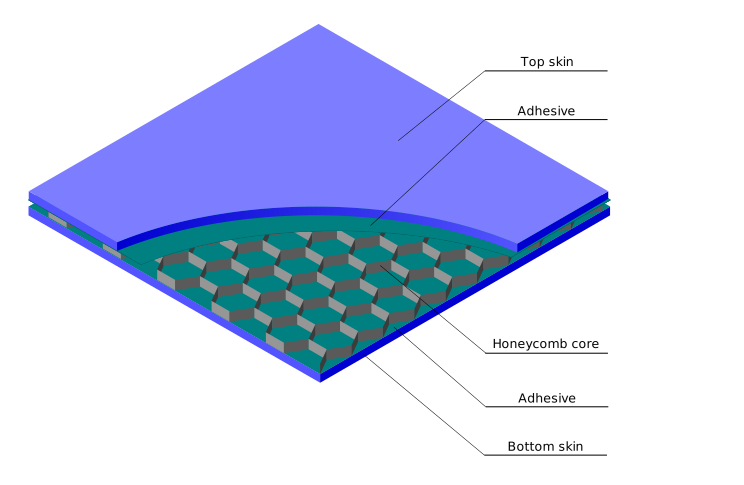
\includegraphics[height=4cm]{Intro/honeycomb_plate} \caption{
			\label{fig:hcp} Honeycomb sandwich panel.}
		\vspace{-0.5cm}
	\end{center}
\end{figure}
Sandwich structures consist of facings of materials with good mechanical properties separated by a core of lightweight materials. The result is, compared to a solid construction of the same density, a similar tensile strength and a significantly higher bending strength. The stresses induced by the bending moment are significantly lower in sandwich construction.

The facings, made of materials with good mechanical properties, are designed to carry tensile or compressive stresses from longitudinal forces and bending moments. The core, on the other hand, transmits mainly shear stresses from transverse forces. It also separates the cladding from each other, which increases structural stiffness for thin cladding, improves insulation properties, and reduces weight while maintaining strength properties similar to solid construction.


However, these complex structures are exposed to various types of damage that are not found in metal alloy materials, e.g., hidden disbonds between the skin and the core, delamination of the skin plates, or the core impact damage.
They can occur either during a manufacturing process, storage or in-service life.
Therefore, advanced methods are required for on-line damage detection.




However, these complex structures are exposed to a risk of different types of failures such as delamination, cracks, disbonds, poor cure and voids, which can occur either during a manufacturing process, storage or in-service life.
Thus, the use of composites has forced the development of advanced approaches to structural inspections. 
 However, these complex structures are exposed to a risk of different types of failures such as delamination, cracks, disbonds, poor cure and voids. Defects can occur either during a manufacturing process, storage or in--service life.
